\documentclass[
	english,
	fontsize=10pt,
	parskip=half,
	titlepage=true,
	DIV=12
]{scrartcl}

\usepackage[utf8]{inputenc}
\usepackage{babel}
\usepackage[T1]	{fontenc}
\usepackage{lmodern}
\usepackage{microtype}
\usepackage{color}
\usepackage{csquotes}

\usepackage{hyperref}

\newcommand*{\tabcrlf}{\\ \hline}

\usepackage{amsmath}
\usepackage{amssymb}
\usepackage{dsfont}
\usepackage[arrowdel]{physics}
\usepackage{mathtools}
\usepackage{siunitx}

\usepackage{minted}
	\usemintedstyle{friendly}

\newcommand*{\inPy}[1]{\mintinline{python}{#1}}
\newcommand*{\ie}{i.\,e.}
\newcommand*{\eg}{e.\,g.}

\begin{document}

\part*{Python Problems 01, Summer 2021}

\section{Time Complexity (1)}
The below code shows an implementation of the selection sort algorithm. Analyze its time complexity (Big O Notation).
\begin{minted}[linenos]{python3}
def selectionSort(data) :
    for k in range(len(data)) :
        x, i = min([(x, i) for (i, x) in enumerate(data[k:])])
        data[k], data[k + i] = data[k + i], data[k]    
\end{minted}

\section{Time Complexity (2)}
The matrix multiplication is usually implemented in $\mathcal{O}(N^3)$ (we implicitly assume square matrixes of size $N \times N$ here). There are a few algorithms that are nominally better, but they are hardly fit for practice.\\
Can you give a simple argument why, no matter how smart it is done, there can be no algorithm that performs matrix multiplication faster than $\mathcal{O}(N^2)$?

\section{Time Complexity (3)}
The below code shows a recursive implementation of computing the factorial ($N!$) of an integer $N$. Why can we not use the master theorem here to find the time complexity? Try to assess the time complexity anyway.
\begin{minted}[linenos]{python3}
def factorial(N) :
    if type(N) != int :
        raise TypeError("factorial can only be computed for ints!")
    if N < 0 :
        raise ValueError("factorial can only be computed for positive ints!")
    elif N == 0 :
        return 1
    else :
        return N * factorial(N - 1)
\end{minted}

Why is the following implementation by far superior?
\begin{minted}[linenos]{python3}
def factorial(N) :
    if type(N) != int :
        raise TypeError("factorial can only be computed for ints!")
    if N < 0 :
        raise ValueError("factorial can only be computed for positive ints!")
    
    reVal = N
    for i in range(1, N) :
        reVal *= i
    return reVal
\end{minted}

\section{Time Complexity (4)}
Use the Master Theorem to analyze the time complexity of this algorithm that computes the sum of an array:
\begin{minted}[linenos]{python3}
def listRecSum (data, start=0, end=-1) :
    
    if end < 0 : 
        L = len(data)
        end = L
    else :
        L = end - start
    
    if L == 1 :
        return data[start]
    elif L == 2 :
        return data[start] + data[end - 1]
    else :
        midPoint = start + L // 2
        return listRecSum(data, start, midPoint) + listRecSum(data, midPoint, end)

data = list(range(11))
print( listRecSum(data) )    # output: 55
\end{minted}

\section{Data Base Queries}
Imagine you are maintaining a database like the one below:
\begin{minted}{text}
  ID   |  last name  | first name | sex |  department  | join date
-------+-------------+------------+-----+--------------+------------
561813 | Atreides    | Siona      |  F  | intelligence | 2005-09-01
886482 | Tivrusky IV | Edward     |  F  | IT           | 2012-12-01
186181 | Mustang     | Roy        |  M  | intelligence | 1989-03-29
...
\end{minted}

Assume that internally, last and first name are represented as strings, sex is represented as a boolean, department is an integer (\ie department ID) and join date is an interger, too (days since some \enquote{epoch date}). The database as a whole is available as a \inPy{list} of \inPy{dict}s.

Write (pseudo-)code that returns the IDs of all women in the IT intelligence department whose last name starts with an A and who joined after 2005. Think about lazy evaluation to formulate this query in an efficient to evaluate way.

\section{Lazy Monte Carlo Integral}
Evaluate the following integral:
\[
	\int_{-16}^{+16} \dd{x}
	\int_{-16}^{+16} \dd{y} \;
		\exp[-0.1 (x^2 + y^2)]
		\qty|
			\sin(5 x) + \cos(0.5 y)
		|
\]

First do it naively, \ie evaluate it for each coordinate pair $(x, y)$ where $x \in [-16, +16]$ and $y \in [-16, +16]$, with a given resolution, \eg $\Delta x = \Delta y = 0.02$. That means, evaluate for
\[ (x, y) \in \{(-16.00, -16.00), (-15.98, -16.00), (-15.96, -16.00), \ldots, (-16.00, -15.98), \ldots, (+16.00, +16.00) \} \]

Measure the time this takes with the \texttt{time.time()} function.

\emph{Hint}:\\
On my machine, this took about \SI{200}{ms}. If you measure repeatedly to incresase accuracy, don't overdo it ;)

\emph{Hint}:\\
Use \texttt{numpy} to speed things up a little bit.

\emph{Hint}:\\
If I did it right, the result should be very close to 25.

Now look at this plot of the function we integrate over:
\begin{center}
	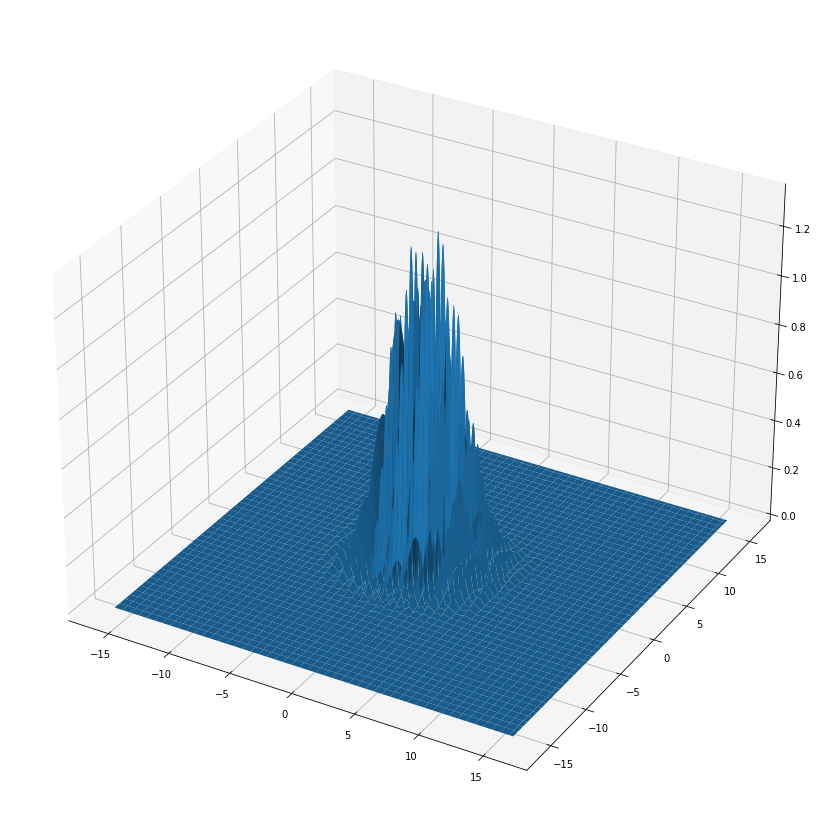
\includegraphics[width=0.6\linewidth]{func}
\end{center}

We see that the function is close to zero everywhere outside a certain cutoff radius $r_c$. In other words, we can safely neglect such points $(x, y)$ where
\[ x^2 + y^2 > r_c^2 \]

When the integrand takes long to evaluate, we often apply \emph{Monte Carlo Methods}. In the simplest case, this means we select random spots to evaluate the function. We then evaluate the function only in these \emph{few}, randomly chosen spots and weight them each with $\frac{\text{total area}}{N}$ where $N$ is the number of random spots chosen and \emph{total area} is the area that we're integrating over.

Implement this Monte Carlo approach and use lazy evaluation to further reduce the effort. Again, measure the time this takes using \texttt{time.time()}. Compare your results wrt. both, time taken and accuracy.

\emph{Hint}:\\
The error of Monte Carlo Methods goes like $\frac{1}{\sqrt{N}}$. That means if you increase the number of sampled points $N$ by a factor of 100, your error should go down by a factor of 10.

\emph{Hint}:\\
I got a speedup of almost 25x while staying within within $\pm 0.8\%$ of the \enquote{exact} result. Can you beat me to that?
\end{document}

